\documentclass[a4paper,11pt]{report}

\usepackage{amsmath,amssymb}
\usepackage{fullpage}
\usepackage{graphicx}

\usepackage{bussproofs}
\usepackage{mathpartir}
\usepackage{prooftrees}
\usepackage{color}

\usepackage{tikz}
\usetikzlibrary{automata,positioning}

\newcommand*\circled[1]{\tikz[baseline=(char.base)]{
            \node[shape=circle,draw,inner sep=2pt] (char) {#1};}}

\makeatletter
\pgfmathdeclarefunction{alpha}{1}{%
  \pgfmathint@{#1}%
  \edef\pgfmathresult{\pgffor@alpha{\pgfmathresult}}%
}

\newcommand*{\until}{U}
\newcommand*{\disj}{\ ,\ }
\newcommand*{\A}{\square}  % Always
\newcommand*{\D}{\diamondsuit} % eventually

\newcommand*{\Pq}{(\top,\bot)}
\newcommand*{\pQ}{(\bot,\top)}
\newcommand*{\PQ}{(\top,\top)}
\newcommand*{\pq}{(\bot,\bot)}

% tikz
\usepackage{tikz}
\usetikzlibrary{snakes}

\author{Sylvain Julmy}
\date{\today}

\setlength{\parindent}{0pt}
\setlength{\parskip}{2.5pt}

\begin{document}

\begin{center}
\Large{
    Automata on Infinite Structure\\
    Fall 2018
  }
  
  \noindent\makebox[\linewidth]{\rule{\linewidth}{0.4pt}}
  Exercice Sheet 1

  \vspace*{1.4cm}

  Author : Sylvain Julmy
  \noindent\makebox[\linewidth]{\rule{\linewidth}{0.4pt}}

  \begin{flushleft}
    Professor : Ultes-Nitsche Ulrich
    
    Assistant : Stammet Christophe
  \end{flushleft}

  \noindent\makebox[\linewidth]{\rule{\textwidth}{1pt}}
\end{center}

\section*{Exercice 1}

\begin{align*}
  \mathcal{L}(A_1) &= (b|a)^*a^+\\ 
  \mathcal{L}(A_2) &= a(ba)^* | b(ba)^* | (ab)^* | (ba)^*\\ 
  \mathcal{L}_\omega(A_1) &= b^* (ab^*)^\omega\\ 
  \mathcal{L}\omega(A_2) &= (ab)^\omega | (ba)^\omega
\end{align*}

\section*{Exercice 2}

\subsection*{1.}

\begin{center}
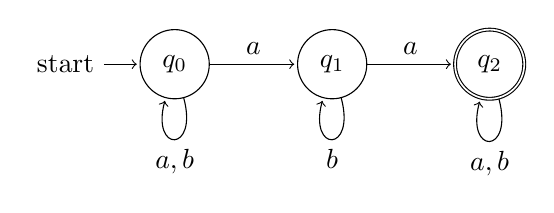
\begin{tikzpicture}[shorten >=1pt,node distance=2cm,on grid,auto]
  \node[state,initial] (q0) {$q_0$};
  \node[state] (q1) [right = of q0] {$q_1$};
  \node[state,accepting] (q2) [right = of q1] {$q_2$};
  \path[->]
  (q0)
  edge [loop below] node [] {$a,b$} ()
  edge [] node [] {$a$} (q1)
  (q1)
  edge [loop below] node [] {$b$} ()
  edge [] node [] {$a$} (q2)
  (q2)
  edge [loop below] node [] {$a,b$} ()
  ;
\end{tikzpicture}
\end{center}

\subsection*{2.}

\begin{center}
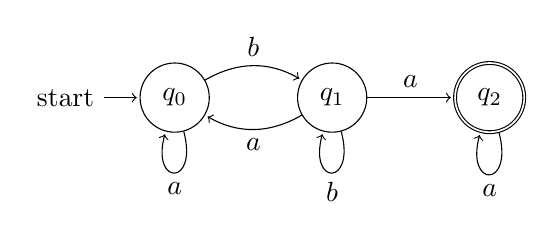
\begin{tikzpicture}[shorten >=1pt,node distance=2cm,on grid,auto]
  \node[state,initial] (q0) {$q_0$};
  \node[state] (q1) [right = of q0] {$q_1$};
  \node[state,accepting] (q2) [right = of q1] {$q_2$};
  \path[->]
  (q0)
  edge [loop below] node [] {$a$} ()
  edge [bend left] node [] {$b$} (q1)
  (q1)
  edge [loop below] node [] {$b$} ()
  edge [] node [] {$a$} (q2)
  edge [bend left] node [] {$a$} (q0)
  (q2)
  edge [loop below] node [] {$a$} ()
  ;
\end{tikzpicture}
\end{center}

\subsection*{3.}

To construct such an automata, we have to create state which uniquely check
every possible sequence of appearence of the letter from $\Sigma$. The number of
different sequence is $n = 2^{|\Sigma|} = 2^{26} = 67'108'864$, as said during
the exerice classes.

To do the construction :
\begin{enumerate}
\item Create an initial state $q_0$ with transition to $|\Sigma|$ other state
  $q_i, i \in [1;|\Sigma|]$ labelled with each letters of the alphabet. Each of
  those state check the presence of one specific letter.
\item For each of those state, we add $|\Sigma|-1$ transition to another
  $|\Sigma|-1$ states labeled $q_{i,j}$ where $j \in [1;|\Sigma|-1]$. To check
  the second letter.
\item We repeat $1$ and $2$ until every possible sequence is recognize.
\item Each state as a transition to itself with all the letters which is
  previusly recognize by the run.
\end{enumerate}


\end{document}